\documentclass[
  shownotes,
  xcolor={svgnames},
  hyperref={colorlinks,citecolor=DarkBlue,linkcolor=DarkRed,urlcolor=DarkBlue}
  , aspectratio=169]{beamer}
\usepackage{animate}
\usepackage{amsmath}
\usepackage{amsfonts}
\usepackage{amssymb}
\usepackage{pifont}
\usepackage{mathpazo}
%\usepackage{xcolor}
\usepackage{multimedia}
\usepackage{fancybox}
\usepackage[para]{threeparttable}
\usepackage{multirow}
\setcounter{MaxMatrixCols}{30}
\usepackage{subcaption}
\usepackage{graphicx}
\usepackage{lscape}
\usepackage[compatibility=false,font=small]{caption}
\usepackage{booktabs}
\usepackage{ragged2e}
\usepackage{chronosys}
\usepackage{appendixnumberbeamer}
\usepackage{animate}
\setbeamertemplate{caption}[numbered]
\usepackage{color}
%\usepackage{times}
\usepackage{tikz}
\usepackage{comment} %to comment
%% BibTeX settings
\usepackage{natbib}
\bibliographystyle{apalike}
\bibpunct{(}{)}{,}{a}{,}{,}
\setbeamertemplate{bibliography item}{[\theenumiv]}

% Defines columns for bespoke tables
\usepackage{array}
\newcolumntype{L}[1]{>{\raggedright\let\newline\\\arraybackslash\hspace{0pt}}m{#1}}
\newcolumntype{C}[1]{>{\centering\let\newline\\\arraybackslash\hspace{0pt}}m{#1}}
\newcolumntype{R}[1]{>{\raggedleft\let\newline\\\arraybackslash\hspace{0pt}}m{#1}}


\usepackage{xfrac}


\usepackage{multicol}
\setlength{\columnsep}{0.5cm}

% Theme and colors
\usetheme{Boadilla}

% I use steel blue and a custom color palette. This defines it.
\definecolor{andesred}{HTML}{af2433}

% Other options
\providecommand{\U}[1]{\protect\rule{.1in}{.1in}}
\usefonttheme{serif}
\setbeamertemplate{itemize items}[default]
\setbeamertemplate{enumerate items}[square]
\setbeamertemplate{section in toc}[circle]

\makeatletter

\definecolor{mybackground}{HTML}{82CAFA}
\definecolor{myforeground}{HTML}{0000A0}

\setbeamercolor{normal text}{fg=black,bg=white}
\setbeamercolor{alerted text}{fg=red}
\setbeamercolor{example text}{fg=black}

\setbeamercolor{background canvas}{fg=myforeground, bg=white}
\setbeamercolor{background}{fg=myforeground, bg=mybackground}

\setbeamercolor{palette primary}{fg=black, bg=gray!30!white}
\setbeamercolor{palette secondary}{fg=black, bg=gray!20!white}
\setbeamercolor{palette tertiary}{fg=white, bg=andesred}

\setbeamercolor{frametitle}{fg=andesred}
\setbeamercolor{title}{fg=andesred}
\setbeamercolor{block title}{fg=andesred}
\setbeamercolor{itemize item}{fg=andesred}
\setbeamercolor{itemize subitem}{fg=andesred}
\setbeamercolor{itemize subsubitem}{fg=andesred}
\setbeamercolor{enumerate item}{fg=andesred}
\setbeamercolor{item projected}{bg=gray!30!white,fg=andesred}
\setbeamercolor{enumerate subitem}{fg=andesred}
\setbeamercolor{section number projected}{bg=gray!30!white,fg=andesred}
\setbeamercolor{section in toc}{fg=andesred}
\setbeamercolor{caption name}{fg=andesred}
\setbeamercolor{button}{bg=gray!30!white,fg=andesred}


\usepackage{fancyvrb}
\newcommand{\VerbBar}{|}
\newcommand{\VERB}{\Verb[commandchars=\\\{\}]}
\DefineVerbatimEnvironment{Highlighting}{Verbatim}{commandchars=\\\{\}}
% Add ',fontsize=\small' for more characters per line
\usepackage{framed}
\definecolor{shadecolor}{RGB}{248,248,248}
\newenvironment{Shaded}{\begin{snugshade}}{\end{snugshade}}
\newcommand{\AlertTok}[1]{\textcolor[rgb]{0.94,0.16,0.16}{#1}}
\newcommand{\AnnotationTok}[1]{\textcolor[rgb]{0.56,0.35,0.01}{\textbf{\textit{#1}}}}
\newcommand{\AttributeTok}[1]{\textcolor[rgb]{0.77,0.63,0.00}{#1}}
\newcommand{\BaseNTok}[1]{\textcolor[rgb]{0.00,0.00,0.81}{#1}}
\newcommand{\BuiltInTok}[1]{#1}
\newcommand{\CharTok}[1]{\textcolor[rgb]{0.31,0.60,0.02}{#1}}
\newcommand{\CommentTok}[1]{\textcolor[rgb]{0.56,0.35,0.01}{\textit{#1}}}
\newcommand{\CommentVarTok}[1]{\textcolor[rgb]{0.56,0.35,0.01}{\textbf{\textit{#1}}}}
\newcommand{\ConstantTok}[1]{\textcolor[rgb]{0.00,0.00,0.00}{#1}}
\newcommand{\ControlFlowTok}[1]{\textcolor[rgb]{0.13,0.29,0.53}{\textbf{#1}}}
\newcommand{\DataTypeTok}[1]{\textcolor[rgb]{0.13,0.29,0.53}{#1}}
\newcommand{\DecValTok}[1]{\textcolor[rgb]{0.00,0.00,0.81}{#1}}
\newcommand{\DocumentationTok}[1]{\textcolor[rgb]{0.56,0.35,0.01}{\textbf{\textit{#1}}}}
\newcommand{\ErrorTok}[1]{\textcolor[rgb]{0.64,0.00,0.00}{\textbf{#1}}}
\newcommand{\ExtensionTok}[1]{#1}
\newcommand{\FloatTok}[1]{\textcolor[rgb]{0.00,0.00,0.81}{#1}}
\newcommand{\FunctionTok}[1]{\textcolor[rgb]{0.00,0.00,0.00}{#1}}
\newcommand{\ImportTok}[1]{#1}
\newcommand{\InformationTok}[1]{\textcolor[rgb]{0.56,0.35,0.01}{\textbf{\textit{#1}}}}
\newcommand{\KeywordTok}[1]{\textcolor[rgb]{0.13,0.29,0.53}{\textbf{#1}}}
\newcommand{\NormalTok}[1]{#1}
\newcommand{\OperatorTok}[1]{\textcolor[rgb]{0.81,0.36,0.00}{\textbf{#1}}}
\newcommand{\OtherTok}[1]{\textcolor[rgb]{0.56,0.35,0.01}{#1}}
\newcommand{\PreprocessorTok}[1]{\textcolor[rgb]{0.56,0.35,0.01}{\textit{#1}}}
\newcommand{\RegionMarkerTok}[1]{#1}
\newcommand{\SpecialCharTok}[1]{\textcolor[rgb]{0.00,0.00,0.00}{#1}}
\newcommand{\SpecialStringTok}[1]{\textcolor[rgb]{0.31,0.60,0.02}{#1}}
\newcommand{\StringTok}[1]{\textcolor[rgb]{0.31,0.60,0.02}{#1}}
\newcommand{\VariableTok}[1]{\textcolor[rgb]{0.00,0.00,0.00}{#1}}
\newcommand{\VerbatimStringTok}[1]{\textcolor[rgb]{0.31,0.60,0.02}{#1}}
\newcommand{\WarningTok}[1]{\textcolor[rgb]{0.56,0.35,0.01}{\textbf{\textit{#1}}}}
\usepackage{graphicx}
\makeatletter


% colors
\definecolor{airforceblue}{rgb}{0.36, 0.54, 0.66}
\newcommand{\theme}{\color{andesred}}
\newcommand{\bk}{\color{black}}
\newcommand{\rd}{\color{red}}
\newcommand{\fg}{\color{ForestGreen}}
\newcommand{\bl}{\color{blue}}
\newcommand{\gr}{\color{black!60}}
\newcommand{\sg}{\color{DarkSlateGray}}
\newcommand{\br}{\color{SaddleBrown}}
\newcommand{\nv}{\color{Navy}}


% common math markups
\newcommand{\bs}[1]{\boldsymbol{#1}}
\newcommand{\mc}[1]{\mathcal{#1}}
\newcommand{\mr}[1]{\mathrm{#1}}
\newcommand{\bm}[1]{\mathbf{#1}}
\newcommand{\ds}[1]{\mathds{#1}}
\newcommand{\indep}{\perp\!\!\!\perp}

% shorthand
\newcommand{\sk}{\vspace{.5cm}}
\newcommand{\R}[1]{{\tt \nv #1}}
\newcommand{\til}{{\footnotesize$\bs{\stackrel{\sim}{}}$}}
\DeclareSymbolFont{extraup}{U}{zavm}{m}{n}
\DeclareMathSymbol{\vardiamond}{\mathalpha}{extraup}{87}


\usepackage{tikz}
% Tikz settings optimized for causal graphs.
\usetikzlibrary{shapes,decorations,arrows,calc,arrows.meta,fit,positioning}
\tikzset{
    -Latex,auto,node distance =1 cm and 1 cm,semithick,
    state/.style ={ellipse, draw, minimum width = 0.7 cm},
    point/.style = {circle, draw, inner sep=0.04cm,fill,node contents={}},
    bidirected/.style={Latex-Latex,dashed},
    el/.style = {inner sep=2pt, align=left, sloped}
}


\makeatother






%%%%%%%%%%%%%%% BEGINS DOCUMENT %%%%%%%%%%%%%%%%%%

\begin{document}
 
\title[Lecture 24]{Lecture 24:  Superlearners \& Text as Data}
\subtitle{Big Data and Machine Learning for Applied Economics \\ Econ 4676}
\date{\today}

\author[Sarmiento-Barbieri]{Ignacio Sarmiento-Barbieri}
\institute[Uniandes]{Universidad de los Andes}


\begin{frame}[noframenumbering]
\maketitle
\end{frame}

%%%%%%%%%%%%%%%%%%%%%%%%%%%%%%%%%%%




%----------------------------------------------------------------------% 

\begin{frame}
\frametitle{Agenda}

\tableofcontents

\end{frame}

%----------------------------------------------------------------------%
\section{Announcements}
%----------------------------------------------------------------------%
\begin{frame}
\frametitle{Announcements}

\begin{itemize}
\item Problem Set 4: Next Friday presentations
\medskip
\item Thursday you need to submit a .csv it at 8:00 pm. 
  \begin{itemize}
    \item Please upload it to your repo don't forget to follow the instructions, if you have questions ask before hand, {\bf not at 7:30pm before submission!} 
    \medskip
    \item The lowest the better the score (smaller loss)
    \medskip
    \item If you forget to send me the number of parameters I'll assign $100,000$
    \medskip
    \item If I can't grab you predictions file from your repo with  \texttt{grep} you won't get credit for the problem set.
    \medskip 
    \item It should be in the \texttt{stores} folder
  \end{itemize}
\medskip
\item I've uploaded the final presentation schedule
\end{itemize}

\end{frame}
%----------------------------------------------------------------------%
\section{Recap: Bagging, Forests, and Boosting}
%----------------------------------------------------------------------%
\begin{frame}[fragile]
\frametitle{ Forests }


\begin{itemize}
  \item We can improve performance a lot using either bootstrap aggregation (bagging), random forests, or boosting.
  \item Bagging \& Random Forests:
    \begin{itemize}
      \item Repeatedly draw bootstrap samples $(X_i^b,Y_i^b)_{i=1}^N$ from the observed sample.
      \item For each bootstrap sample, fit a regression tree $\hat{f}^b(x)$
      \begin{itemize}
        \item Bagging: full sample
        \item Random Forests: subset of predictors $ \sqrt(p)$ (breaks high correlation)
      \end{itemize}
      \item Average across bootstrap samples to get the predictor
      \begin{align}
        \hat{f}_{bag} =\frac{1}{B}\sum_{b=1}^B \hat{f}^b(x)
      \end{align}
\item Basically we are smoothing predictions. 
\end{itemize}

\end{itemize}
\end{frame}
%----------------------------------------------------------------------%
\begin{frame}[fragile]
\frametitle{Boosting Trees}


\begin{itemize}
\item Learning tree structure is much harder than traditional optimization problem where you can simply take the gradient. 
\item It is intractable to learn all the trees at once. 
\item Instead, we use an additive strategy: fix what we have learned, and add one new tree at a time. We write the prediction value at step m as $\hat{y}_i^{m}$. 
\item Then we have
\begin{align}
\hat{y}_i^{0} &=0 \\ \nonumber
\hat{y}_i^{1} &= \hat{y}_i^{0} + f_1(x_i) \\ \nonumber
\hat{y}_i^{2} &= \hat{y}_i^{1} + f_2(x_i) \\ \nonumber
\dots \\ \nonumber
\hat{y}_i^{M} &= \sum_{m=1}^M f_m(x_i) = \hat{y}_i^{m-1} + f_m(x_i) \\ \nonumber
\end{align}
\end{itemize}


 \end{frame}
%----------------------------------------------------------------------%
\begin{frame}[fragile]
\frametitle{XGBoost is a Boosting Tree }

\begin{itemize}


\item Which tree do we want at each step? 
\item Add the one that optimizes our objective.

\begin{align}
\mathcal{L} &= \sum_{i=1}^N L(y_i,\hat{y}_i) + \sum_{k=1}^m \Omega(f_k)
\end{align}

\item  $L(.)$ is a differentiable convex loss function that measures the difference between the prediction $\hat{y}_i$ and the target $y_i$. 
\item  The second term $\Omega(f)$ penalizes the complexity of the model, where


\begin{align}
\Omega(f)=\gamma T + \frac{1}{2}\lambda ||\omega||_2
\end{align}

\end{itemize}
\end{frame}

%----------------------------------------------------------------------%
\section{Superlearners}
%----------------------------------------------------------------------%
\begin{frame}[fragile]
\frametitle{}


\centering
{\huge \textcolor{andesred}{Superlearners}}


\end{frame}
%----------------------------------------------------------------------%
\begin{frame}[fragile]
\frametitle{Superlearnes: Motivation}

\begin{itemize}


\item Superlearning is a technique for prediction that involves combining many individual statistical algorithms  to create a new, single prediction algorithm that is expected to perform at least as well as any of the individual algorithms.
\medskip
\item The inovation?
\pause
\medskip
\item The superlearner algorithm “decides” how to combine, or weight, the individual algorithms based upon how well each one minimizes a specified loss function
\medskip
\item The motivation for this type of “ensembling” is that a mix of multiple algorithms may be more optimal for a given data set than any single algorithm. 
\medskip
\item For example, a tree based model averaged with a linear model (e.g. random forests and LASSO) could smooth some of the model’s edges to improve predictive performance.
\end{itemize}

\end{frame}
%----------------------------------------------------------------------%
\begin{frame}[fragile]
\frametitle{Superlearnes: Algorithm}

\begin{itemize}
  \item We have some data $(y_i,X_i)$
  \medskip
\item The goal here is to solve something which looks like
\begin{align}
f^\star=\underset{f\in\mathcal{F}}{\text{argmin}}\left\lbrace \sum_{i=1}^n L(y_i,f({X}_i)) \right\rbrace
\end{align}


\item for some loss function $L$, which is more often than not the  squared error loss, L2 : $(y_i-f{X}_i)^2$ 
\medskip
\item For a given problem, a library of prediction algorithms can be proposed. 
\medskip
\item A library is simply a collection of algorithms.
\end{itemize}
\end{frame}
%----------------------------------------------------------------------%
\begin{frame}[fragile]
\frametitle{Superlearnes: Algorithm}
Denote the library $\mathcal{L}$ and its cardinality as $V(n)$.

\medskip 
 \begin{enumerate}
 \item Fit each algorithm in $\mathcal{L}$ on the entire data set $X = \{X_i : i = 1,...,n\}$ to estimate $f_v(X)$ with $v=1,\dots,V(n)$
 \medskip
 \item  Split the data set $X$ into a training and validation sample, according to a K-fold cross-validation scheme: 
 \medskip
\begin{itemize}
  \item Splits the ordered n observations into K-equal size groups, 
  \begin{itemize}
  \item let the k-th group be the validation sample, 
  \item and the remaining group the training sample
  \end{itemize}
  \item  Define $T(k)$ to be the kth training data split and $Te(k)$ to be the corresponding validation data split. $T(k)=X\slash V(k),k=1,...,K.$
\end{itemize}
  
 \end{enumerate}

\end{frame}
%----------------------------------------------------------------------%
\begin{frame}[fragile]
\frametitle{Superlearnes: Algorithm}


 
 \begin{enumerate}
 \setcounter{enumi}{2}
 \item For the kth fold, fit each algorithm in $\mathcal{L}$  on $T(k)$ and save the predictions on the corresponding test , $\hat{f}_{k,T}(X_i)$ with $X\in Te(k)$
 \medskip
 \item Bind the predictions from each algorithm together to create a n by V matrix
\end{enumerate}

\end{frame}
%----------------------------------------------------------------------%
\begin{frame}[fragile]
\frametitle{Superlearnes: Algorithm}


 
 \begin{enumerate}
 \setcounter{enumi}{4}
 \item Propose a family of weighted combinations of the candidate estimators indexed by weight-vector $\alpha$:
 \medskip
 \begin{align}
  m(z|\alpha) &= \sum_{v=1}^V \alpha_v \hat{f}(X_i)_v \\ \nonumber
  \alpha_v &\geq 0 \, \forall v \\ 
\sum_{v=1}^V \alpha_v &=1 \nonumber
 \end{align}
\end{enumerate}
\end{frame}

%----------------------------------------------------------------------%
\begin{frame}[fragile]
\frametitle{Superlearnes: Algorithm}



 \begin{enumerate}
   \setcounter{enumi}{5}
   \item Determine the $\alpha$ that minimizes the cross-validated risk of the candidate estimator $\sum_{v=1}^V \alpha_v \hat{f}(X_i)$ over all allowed $\alpha$-combinations:
   \begin{align}
    \hat{\alpha} &=\underset{\alpha}{argmin}\sum_{i=1}^n (y_i - m(z|\alpha))^2
   \end{align}

   \medskip

    \item Combine $\hat{\alpha}_v$ with $\hat{f}_v(X_i)$  according to the weights found, and create the final super learner fit
    \begin{align}
    \hat{f}_{SL}(X) = \sum_{v=1}^V \hat{\alpha}_v\hat{f}_v(X_i) 
    \end{align}
\end{enumerate}

\end{frame}

%----------------------------------------------------------------------%
\begin{frame}[fragile]
\frametitle{Superlearnes: Algorithm}
Some considerations:
\begin{itemize}

\item The super learner theory does not place any restrictions on the family of weighted combinations used for ensembling the algorithms in the library.
\medskip
\item The restriction of the parameter space for $\alpha$ to be the convex combination of the algorithms in the library provides greater stability of the final super learner prediction. 

\medskip
\item Restricting to the convex combination implies that if each algorithm in the library is bounded, the convex combination will also be bounded.
\end{itemize}
\end{frame}
%----------------------------------------------------------------------%
\begin{frame}[fragile]
\frametitle{Superlearnes: Summary}



  \begin{figure}[H] \centering
            \captionsetup{justification=centering}
              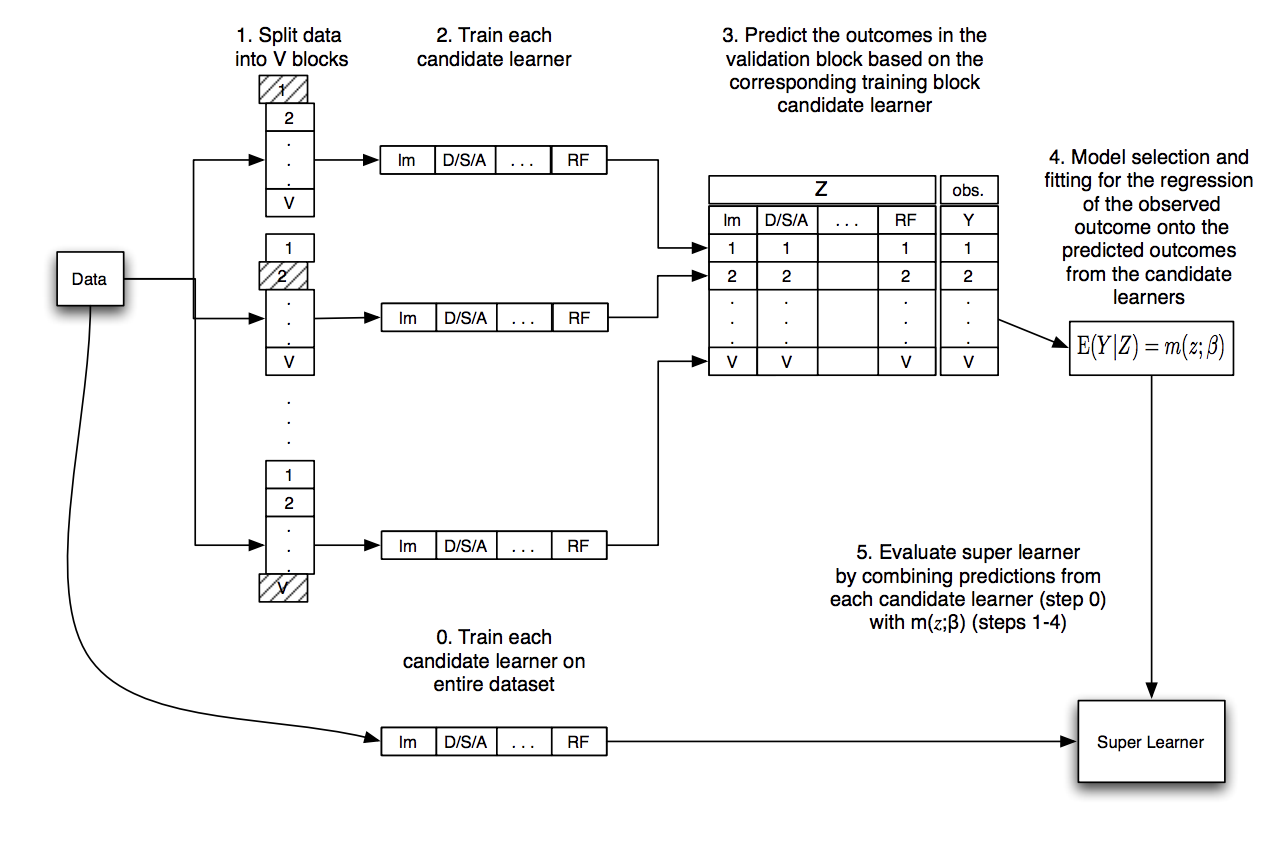
\includegraphics[scale=0.5]{figures/sl_diagram.png}
              \\
              \tiny
              Source: Polley, Eric. Learning: Causal Inference for Observational and Experimental Data
 \end{figure}

\end{frame}
%----------------------------------------------------------------------%
\begin{frame}[fragile]
\frametitle{Superlearnes: Available Learners}



  \begin{figure}[H] \centering
            \captionsetup{justification=centering}
              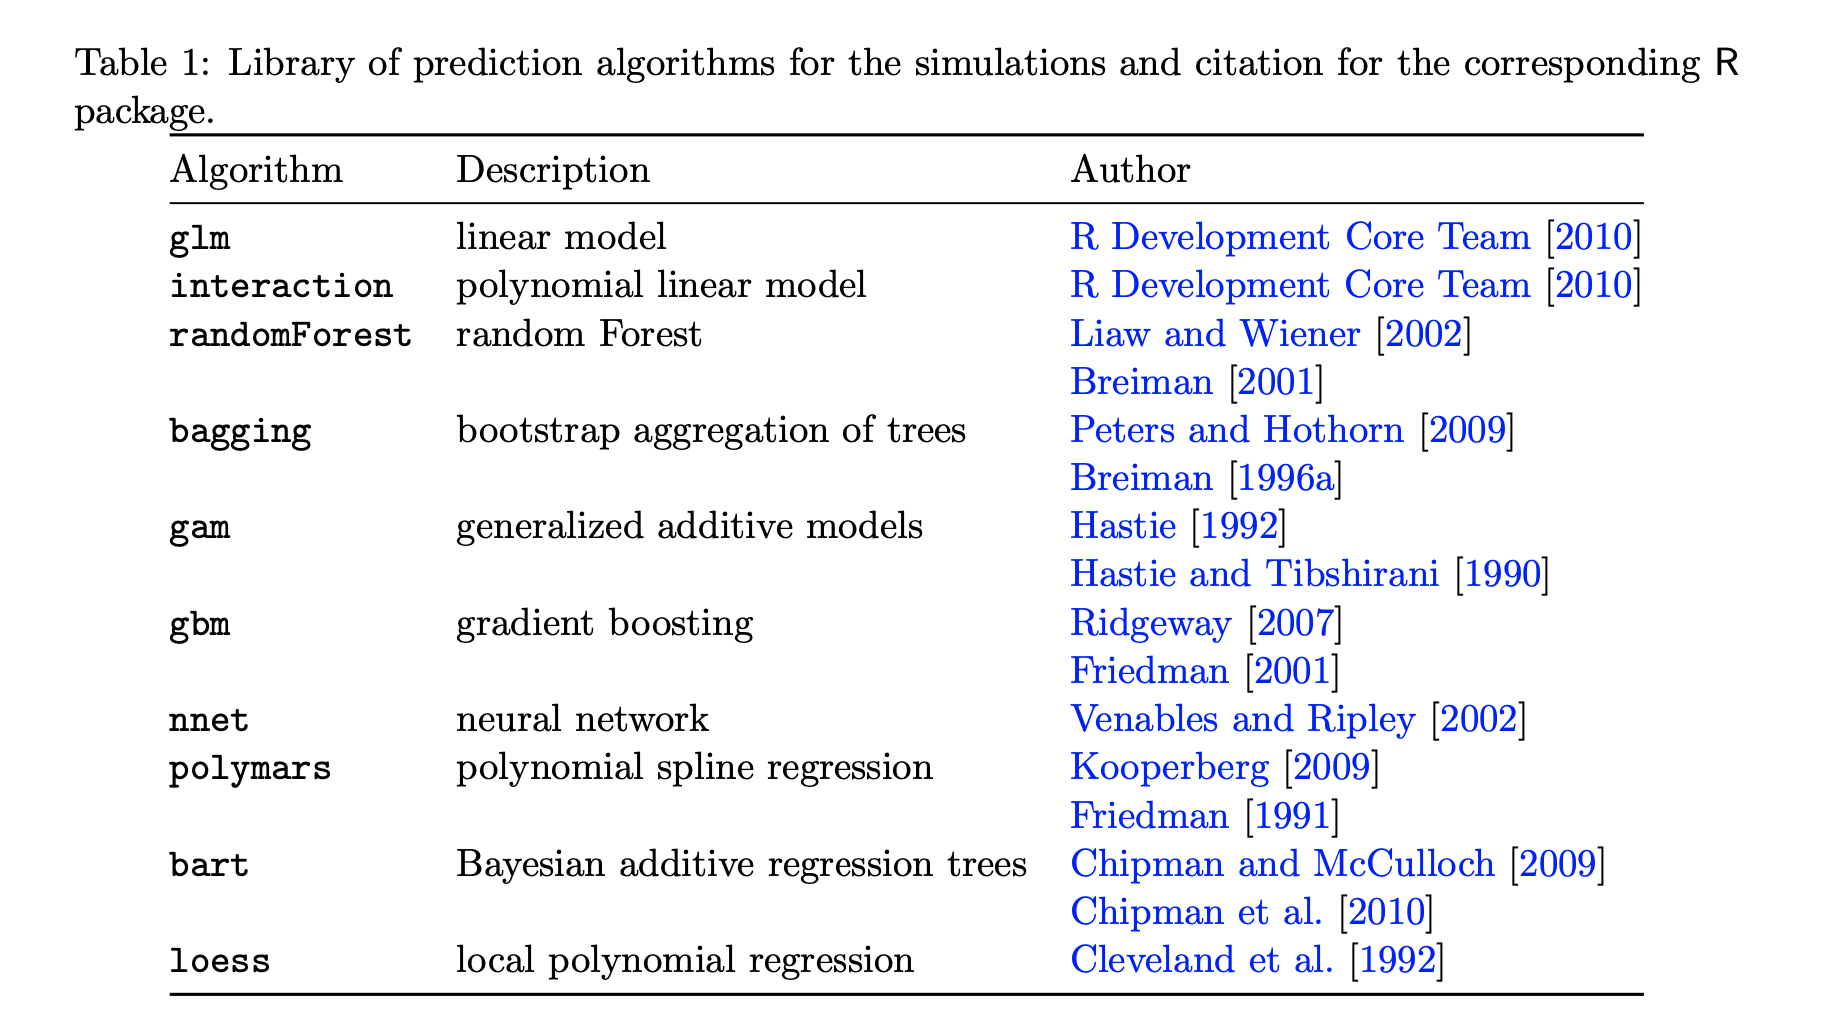
\includegraphics[scale=0.4]{figures/sl_algorithms.png}
              \\
              \tiny
              Source: Polley, Eric. Learning: Causal Inference for Observational and Experimental Data
 \end{figure}

 \end{frame}
%----------------------------------------------------------------------%
\begin{frame}[fragile]
\frametitle{Superlearnes: Performance}



  \begin{figure}[H] \centering
            \captionsetup{justification=centering}
              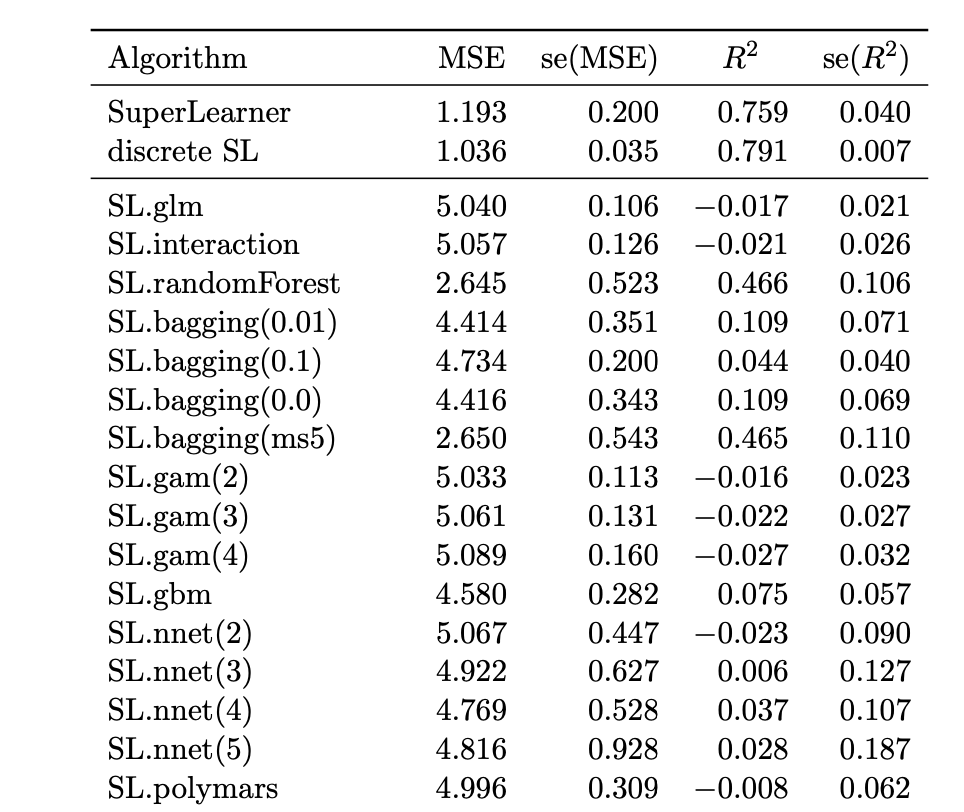
\includegraphics[scale=0.5]{figures/sL_results.png}
              \\
              \tiny
              Source: Polley, Eric. Learning: Causal Inference for Observational and Experimental Data
 \end{figure}


\end{frame}
%----------------------------------------------------------------------%
\section{Text as Data}
%----------------------------------------------------------------------%
\begin{frame}[fragile]
\frametitle{}


\centering
{\huge \textcolor{andesred}{Text as Data}}


\end{frame}

%----------------------------------------------------------------------%
\begin{frame}[fragile]
\frametitle{Text as Data: The Big Picture}

\begin{itemize}


\item {\bf \theme Text is a vast source of data for business }
\medskip
\item It comes connected to interesting ``author'' variables 
\medskip
  \begin{itemize}
  \item What you buy, what you watch, your reviews
  \medskip
  \item Group membership, who you represent, who you email
  \medskip
  \item Market behavior, macro trends, the weather
  \end{itemize}
\medskip
 
\item Opinion, subjectivity, etc.
\medskip
\item  Sentiment is {\it very} loosely defined:  Observables linked to the variables motivating language choice
\end{itemize}

\end{frame}

%----------------------------------------------------------------------%
\begin{frame}[fragile]
\frametitle{Text as Data: The Big Picture}

\begin{itemize}

\item {\bf \theme Text is also super high dimensional }

\medskip
\item And it gets higher dimensional as you observe more speech.


\medskip
\item Analysis of  phrase counts is the state of the art (hard to beat).
\end{itemize}
\end{frame}
%----------------------------------------------------------------------%
\begin{frame}[fragile]
\frametitle{Text as Data: Story Time}

{\bf We'll start with a story: \theme Slant in Partisan Speech}

  \begin{figure}[H] \centering
            \captionsetup{justification=centering}
              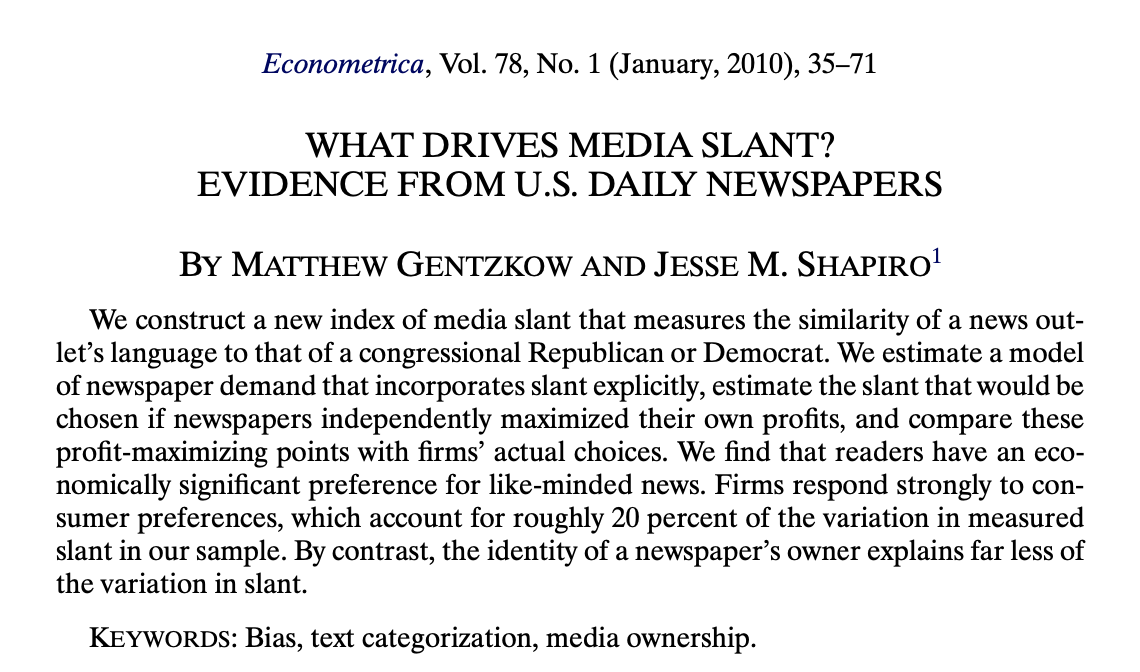
\includegraphics[scale=0.6]{figures/gentzgow_shapiro}
              
 \end{figure}

\end{frame}
%----------------------------------------------------------------------%
\begin{frame}[fragile]
\frametitle{Text as Data: Story Time}
\framesubtitle{Gentzkow and Shapiro: What drives media slant?  Evidence from
U.S. daily newspapers ({\it Econometrica}, 2010)}

\begin{itemize}
\item Build an economic model for newspaper demand that incorporates political partisanship (\rd Republican \bk vs \bl Democrat\bk)


 
\begin{itemize}
\item What would be independent profit-maximizing ``slant''?
\item Compare this to slant estimated from newspaper text.
\end{itemize}
\end{itemize}

\begin{center}
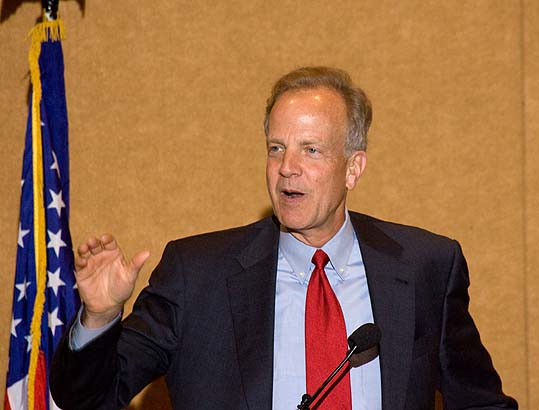
\includegraphics[width=1.7in]{figures/moran}
~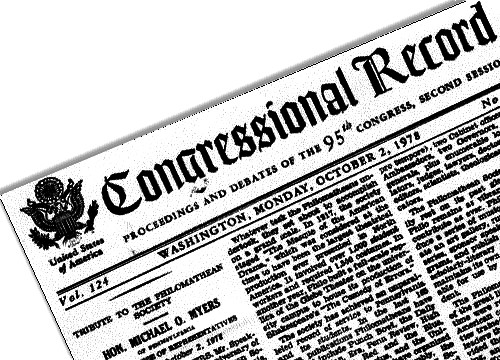
\includegraphics[width=1.75in]{figures/record}
\end{center}


 \end{frame}
%----------------------------------------------------------------------%
\begin{frame}[fragile]
\frametitle{Text as Data: Motivation}

\begin{itemize} 
  \item Jerry Moran, R-KS, says ``death tax'' relatively often and his district (Kansas 1st) voted 73\% for George W. Bush in 2004.

  \item William Jefferson, D-LA, says ``estate tax'' relatively often and his district voted 24\% for George W. Bush in 2004.

\medskip

$\bm{\Rightarrow}$ ``death tax'' is republican



\begin{align}
Ideology = f(\bm{X_\text{text}}) + u
\end{align}

where 
\begin{align}
ideology \approx g(Y_{Bush})
\end{align}

\item Gentzkow and Shapiro apply this logic to build an index of slant that sums across a speaker’s term usage weighted by the direction of slant for each term. 

\end{itemize}


\end{frame}


%----------------------------------------------------------------------%
\subsection{Tokenization}
%----------------------------------------------------------------------%
\begin{frame}[fragile]
\frametitle{Information Retrieval and Tokenization}

\begin{itemize}


\item A passage in `{\it As You Like It}' from Shakepeare:

\medskip

~~~ {\sg All the world's a stage,\\
~~~ and all the men and women merely players:\\
~~~ they have their exits and their entrances;\\
~~~ and one man in his time plays many parts...}


\medskip
\item What the econometrian sees:

\medskip
\vspace{-.4cm}{\sg
\begin{verbatim}
   world stage men women play exit entrance time 
       1     1   2     1    2    1        1    1 
\end{verbatim}}

\medskip
\item This is the {\nv Bag-of-Words} representation of text.
\end{itemize}
\end{frame}

%----------------------------------------------------------------------%
\begin{frame}[fragile]
\frametitle{Possible tokenization steps} 

\begin{itemize}


\item Remove words that are super rare {\gr (in say $<\frac{1}{2}$\%, or $<15\%$ of docs; this is application specific)}.
 For example, if {\nv Argentine} occurs only once, it's useless for comparing documents.


\item Stemming:  `{\nv tax}' $\leftarrow$   taxing,  taxes, taxation, taxable, ... 

{\gr A stemmer cuts words to their root with a mix of rules and estimation.`Porter' is standard for English. }



\item  Remove a list of {\nv stop words} containing  irrelevant tokens.

{\gr ~~~~~If, and, but, who, what, the, they, their, a, or, ...}

{\nv Be careful: one person's stopword is another's key term.}


\item Convert to lowercase, drop numbers, punctuation, etc ...\\
{\gr Always application specific: e.g., don't drop {\tt :-)} from tweets.}
\end{itemize}


\end{frame}


%----------------------------------------------------------------------%
\begin{frame}[fragile]
\frametitle{The $n$-gram language model}

\begin{itemize}

\item An $n$-gram language model is one that describes a dialect through transition probabilities on $n$ consecutive words.

\medskip

\item An {\theme $n$-gram tokenization} counts length-$n$ sequences of words.\\
{\sg A unigram is a word, bigrams are transitions between words.}\\
{\gr e.g., {\tt world.stage}, {\tt stage.men}, {\tt men.women}, {\tt women.play}, ...}

\medskip

\item This can give you rich language data, but be careful: $n$-gram token vocabularies are very high dimensional ($p^n$)
\medskip
\item  More generally, you may have domain specific `clauses' that you wish to tokenize.
\medskip
\item  There is always a trade-off between complexity and generality. 
\medskip
\item {\theme Often best to just count words.}

\end{itemize}


\end{frame}

%----------------------------------------------------------------------%
\begin{frame}[fragile]
\frametitle{Text as Data: Wordle} 

\begin{itemize}
  \item {\theme Often best to just count words.}
  \medskip
  \item For example, occurrences by party for some partisan terms

  \vskip .25cm
  {\footnotesize
  \begin{tabular}{|c|c|c|c|c|c|c}
  Congress & State & Party & America & Death Tax & Estate Tax & $\cdots$
  \\ \hline
  \multirow{2}{*}{63} & \multirow{2}{*}{\sf NM} & {\sf dem}  & 108 &
    30 & 140 & \\ &
  & {\sf gop}  & 100 &
    220 & 12  &
  \end{tabular}}

\begin{figure}[H] \centering
            \captionsetup{justification=centering}
              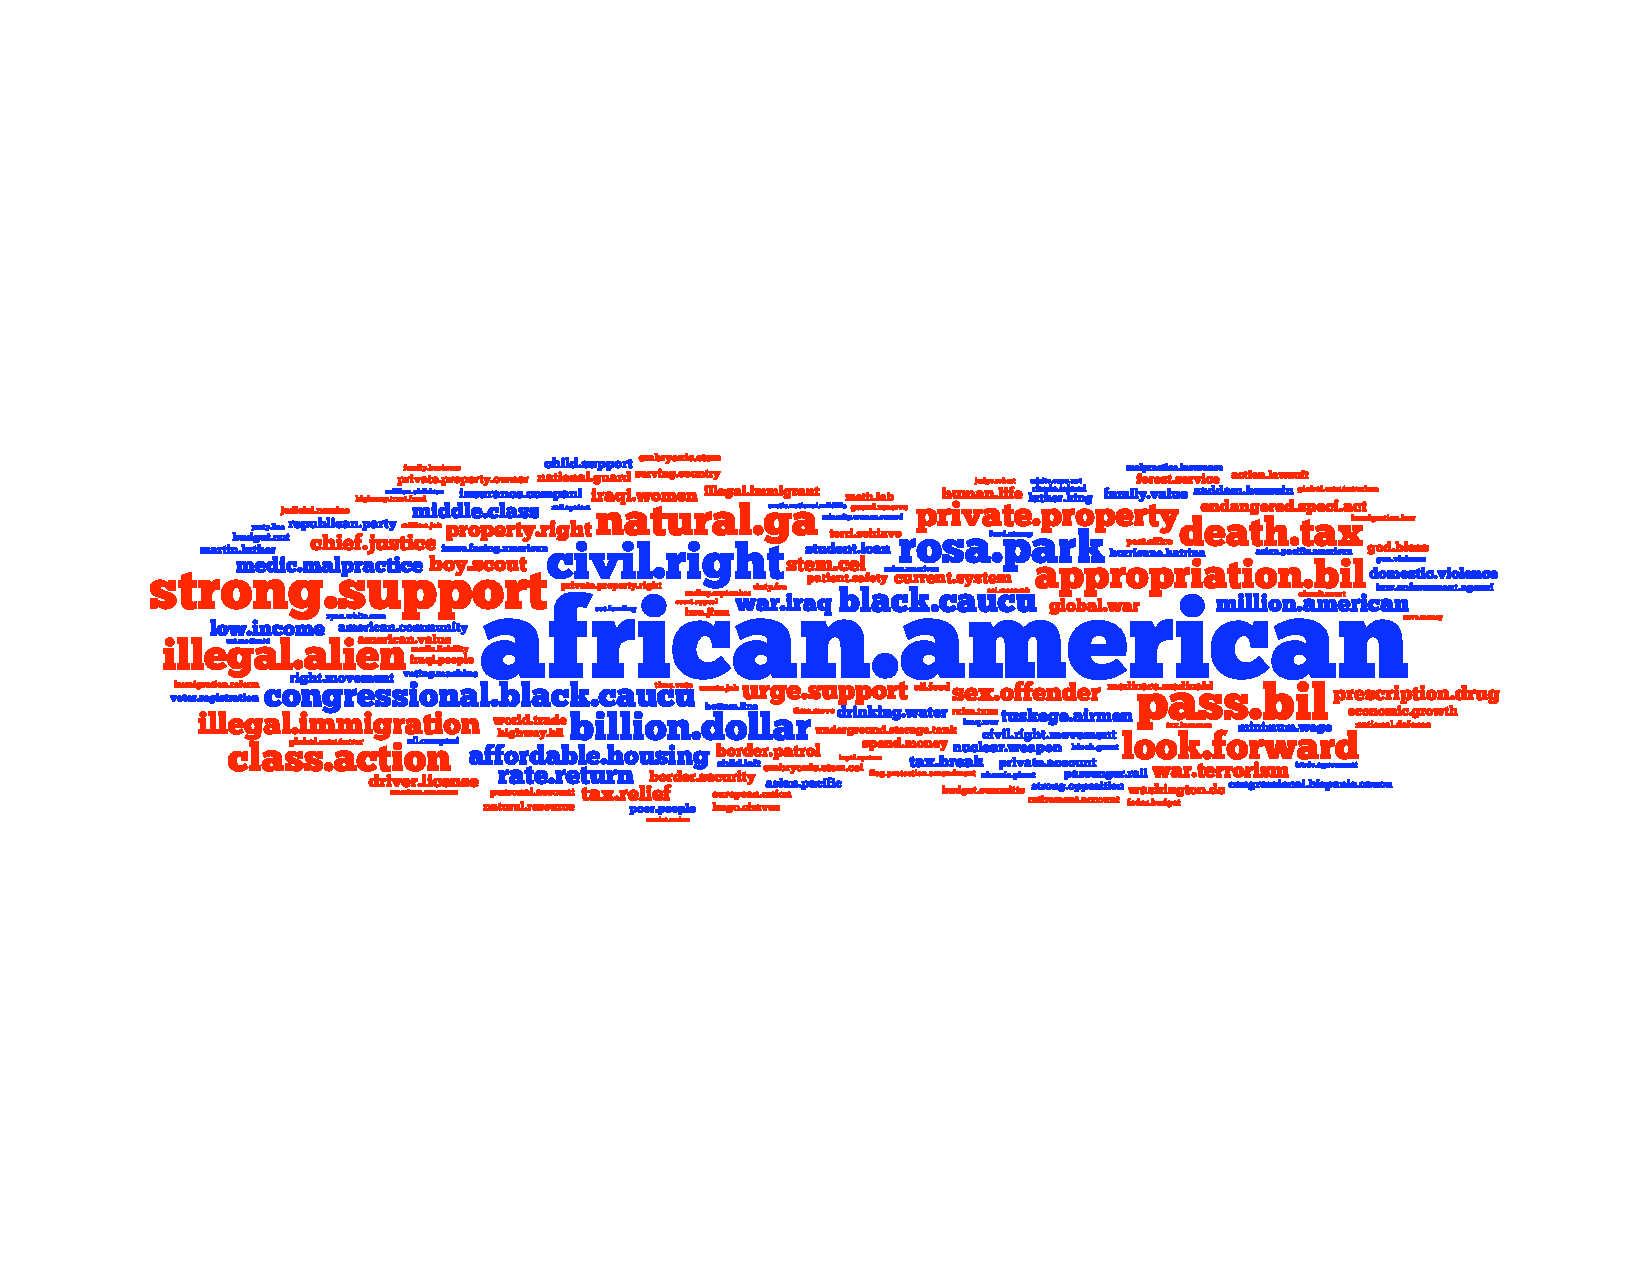
\includegraphics[width=4.5in]{figures/slantWrdl}
              
 \end{figure}

\end{itemize}



\end{frame}
%----------------------------------------------------------------------%
\begin{frame}
\frametitle{Text Regression}

\begin{itemize}
\item Once you have text in a numeric format, we can use all the tools we learned so far

\medskip
\begin{align}
y= f(word\,counts) + u
\end{align}
 
\item where you can use lasso, PCA, etc. to do dimentionality reduction

\end{itemize}
\end{frame}
%----------------------------------------------------------------------%
\begin{frame}
\frametitle{Text Regression}

\begin{center}
{\bf Slant measure for speakers in the 109th Congress}
\vskip -.5cm
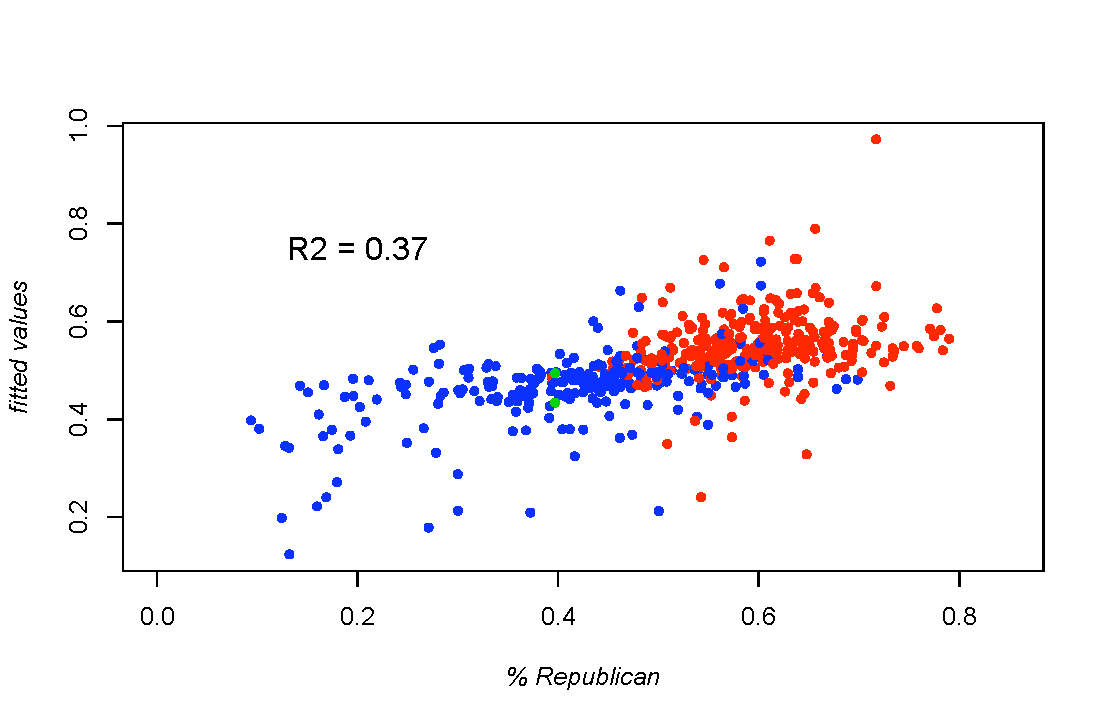
\includegraphics[width=4in]{figures/slant}\\
\end{center}

\vskip -.5cm
Democrats get low $z_\text{slant}$ and Republicans get high
$z_\text{slant}$.\\
\gr Do this for newspaper text and you'll get a similar picture

\end{frame}
%----------------------------------------------------------------------%
\begin{frame}
\frametitle{Text Regression}


\begin{itemize}
\item Another example: Classify emails into spam

\begin{figure}[H] \centering
            \captionsetup{justification=centering}
              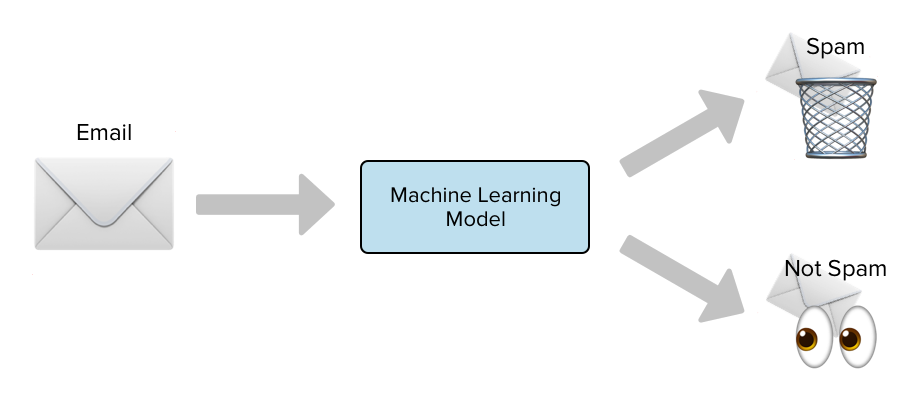
\includegraphics[scale=.2]{figures/spam}
              
 \end{figure}

\medskip
\begin{align}
\mr{logit}\left[{\tt spam} \right] = \alpha + f \beta
\end{align}
\item where $f_i=\frac{x_i}{\sum_j x_{ij}}$ are the normalized text counts
\end{itemize}
\end{frame}
%----------------------------------------------------------------------%
\section{Review  \& Next Steps}
%----------------------------------------------------------------------%
\begin{frame}
\frametitle{Review \& Next Steps}
  
\begin{itemize} 

\item Superlearners
\medskip  
\item Text as Data: Intro

    \bigskip  
  \item  Next class:  More on text as data, dimention reduction, and lots of Linear Algebra!!!


\bigskip  
\item Questions? Questions about software? 

\end{itemize}
\end{frame}


%----------------------------------------------------------------------%
\section{Further Readings}
%----------------------------------------------------------------------%
\begin{frame}
\frametitle{Further Readings}

\begin{itemize}

  \item MJ Van der Laan, EC Polley, AE Hubbard, Super Learner, Statistical applications in genetics and molecular, 2007

  \medskip
  \item Polley, Eric. Learning: Causal Inference for Observational and Experimental Data, by M. J. van der. Laan and Sherri Rose, Springer, 2011.
  \medskip
  \item Polley E, LeDell E, Kennedy C, van der Laan M. Super Learner: Super Learner Prediction. 2016 URL https://CRAN.R-project.org/package=SuperLearner. R package version 2.0-22.
  \medskip
  \item Hoffman, K.. Become a Superlearner! An Illustrated Guide to Superlearning. \url{https://www.khstats.com/blog/sl/superlearning/}
  \medskip
  \item Taddy, M. (2019). Business data science: Combining machine learning and economics to optimize, automate, and accelerate business decisions. McGraw Hill Professional.

  
\end{itemize}

\end{frame}
%----------------------------------------------------------------------%
\section{Appendix: Text as Data Demo}
%----------------------------------------------------------------------%
\subsection{Tokenization Demo}
%----------------------------------------------------------------------%
\begin{frame}[fragile]
\frametitle{Tokenization Demo}

\begin{scriptsize}


\begin{Shaded}
\begin{Highlighting}[]
\CommentTok{\#\# the tm library (and related plugins) is R\textquotesingle{}s ecosystem for text mining.}
\CommentTok{\#\# for an intro see http://cran.r{-}project.org/web/packages/tm/vignettes/tm.pdf}
\KeywordTok{library}\NormalTok{(tm) }
\NormalTok{notes\textless{}{-}}\KeywordTok{readPDF}\NormalTok{(}\DataTypeTok{control =} \KeywordTok{list}\NormalTok{(}\DataTypeTok{text =} \StringTok{"{-}layout {-}enc UTF{-}8"}
  \NormalTok{))(}\DataTypeTok{elem=}\KeywordTok{list}\NormalTok{(}\DataTypeTok{uri=}\StringTok{"\textasciitilde{}/Papers/Beauty\_Hamermesh.pdf"}\NormalTok{), }\DataTypeTok{id=}\NormalTok{fname, }
  \DataTypeTok{language=}\StringTok{\textquotesingle{}en\textquotesingle{}}\NormalTok{)}
writeLines(content(notes)[1]) 
\end{Highlighting}
\end{Shaded}
\end{scriptsize}
\begin{tiny}



\begin{verbatim}
     ARTICLE IN PRESS
                                  Economics of Education Review 24 (2005) 369–376
                                                                                               www.elsevier.com/locate/econedurev
Beauty in the classroom: instructors’ pulchritude and putative
                                         pedagogical productivity
                                     Daniel S. Hamermesh, Amy Parker
                              Department of Economics, University of Texas, Austin, TX 78712-1173, USA
                                            Received 14 June 2004; accepted 21 July 2004
Abstract
   Adjusted for many other determinants, beauty affects earnings; but does it lead directly to the differences in
productivity that we believe generate earnings differences? We take a large sample of student instructional ratings for a
group of university teachers and acquire six independent measures of their beauty, and a number of other descriptors of
them and their classes. Instructors who are viewed as better looking receive higher instructional ratings, with the impact
of a move from the 10th to the 90th percentile of beauty being substantial. This impact exists within university
departments and even within particular courses, and is larger for male than for female instructors. Disentangling
whether this outcome represents productivity or discrimination is, as with the issue generally, probably impossible.
\end{verbatim}
\end{tiny}
\end{frame}
%----------------------------------------------------------------------%
\begin{frame}[fragile]
\frametitle{Tokenization Demo}

\begin{scriptsize}
\begin{Shaded}
\begin{Highlighting}[]
\KeywordTok{content}\NormalTok{(notes) \textless{}{-}}\KeywordTok{iconv}\NormalTok{(}\KeywordTok{content}\NormalTok{(notes), }\DataTypeTok{from=}\StringTok{"UTF{-}8"}\NormalTok{, }\DataTypeTok{to=}\StringTok{"ASCII"}\NormalTok{, }\DataTypeTok{sub=}\StringTok{""}\NormalTok{)}

\NormalTok{docs \textless{}{-}}\StringTok{ }\KeywordTok{Corpus}\NormalTok{(}\KeywordTok{VectorSource}\NormalTok{(notes))}

\KeywordTok{names}\NormalTok{(docs) \textless{}{-}}\StringTok{ }\KeywordTok{names}\NormalTok{(notes) }

\CommentTok{\#\# you can then do some cleaning here}
\CommentTok{\#\# tm\_map just maps some function to every document in the corpus}
\NormalTok{docs \textless{}{-}}\StringTok{ }\KeywordTok{tm\_map}\NormalTok{(docs, }\KeywordTok{content\_transformer}\NormalTok{(tolower)) }\CommentTok{\#\# make everything lowercase}
\NormalTok{docs \textless{}{-}}\StringTok{ }\KeywordTok{tm\_map}\NormalTok{(docs, }\KeywordTok{content\_transformer}\NormalTok{(removeNumbers)) }\CommentTok{\#\# remove numbers}
\NormalTok{docs \textless{}{-}}\StringTok{ }\KeywordTok{tm\_map}\NormalTok{(docs, }\KeywordTok{content\_transformer}\NormalTok{(removePunctuation)) }\CommentTok{\#\# remove punctuation}
\CommentTok{\#\# remove stopword. } 
\CommentTok{\#\#be careful with this: one\textquotesingle{}s stopwords are anothers keywords.}
\CommentTok{\# you could also do stemming; I don\textquotesingle{}t bother here.}
\NormalTok{docs \textless{}{-}}\StringTok{ }\KeywordTok{tm\_map}\NormalTok{(docs, }\KeywordTok{content\_transformer}\NormalTok{(removeWords), }\KeywordTok{stopwords}\NormalTok{(}\StringTok{"SMART"}\NormalTok{))}

\NormalTok{docs \textless{}{-}}\StringTok{ }\KeywordTok{tm\_map}\NormalTok{(docs, }\KeywordTok{content\_transformer}\NormalTok{(stripWhitespace)) }\CommentTok{\#\# remove excess white{-}space}
\end{Highlighting}
\end{Shaded}


\end{scriptsize}

\end{frame}
%----------------------------------------------------------------------%
\begin{frame}[fragile]
\frametitle{Tokenization Demo}


\begin{scriptsize}

\begin{Shaded}
\begin{Highlighting}[]
\CommentTok{\#\# create a doc{-}term{-}matrix}
\NormalTok{dtm \textless{}{-}}\StringTok{ }\KeywordTok{DocumentTermMatrix}\NormalTok{(docs)}
\NormalTok{dtm }
\end{Highlighting}
\end{Shaded}


\end{scriptsize}
\begin{tiny}



\begin{verbatim}
## <<DocumentTermMatrix (documents: 8, terms: 913)>>
## Non-/sparse entries: 1555/5749
## Sparsity           : 79%
## Maximal term length: 30
## Weighting          : term frequency (tf)
\end{verbatim}

\end{tiny}
\begin{scriptsize}

\begin{Shaded}
\begin{Highlighting}[]
\NormalTok{dtm \textless{}{-}}\StringTok{ }\KeywordTok{removeSparseTerms}\NormalTok{(dtm, }\FloatTok{0.75}\NormalTok{)}
\NormalTok{dtm }
\end{Highlighting}
\end{Shaded}

\end{scriptsize}
\begin{tiny}
\begin{verbatim}
## <<DocumentTermMatrix (documents: 8, terms: 156)>>
## Non-/sparse entries: 650/598
## Sparsity           : 48%
## Maximal term length: 15
## Weighting          : term frequency (tf)
\end{verbatim}
\end{tiny}
\end{frame}
%----------------------------------------------------------------------%
\begin{frame}[fragile]
\frametitle{Tokenization Demo}

\begin{scriptsize}


\begin{Shaded}
\begin{Highlighting}[]
\CommentTok{\#\# You can inspect them:}
\KeywordTok{inspect}\NormalTok{(dtm[}\DecValTok{1}\OperatorTok{:}\DecValTok{5}\NormalTok{,}\DecValTok{1}\OperatorTok{:}\DecValTok{8}\NormalTok{])}
\end{Highlighting}
\end{Shaded}
\end{scriptsize}
\begin{tiny}

\begin{verbatim}
## <<DocumentTermMatrix (documents: 5, terms: 8)>>
## Non-/sparse entries: 26/14
## Sparsity           : 35%
## ...
## Docs academic article beauty becker behavior biddle class classes
##    1        1       1      9      1        1      2     1       1
##    2        2       1      7      0        1      0     5       5
##    3        0       1      6      0        0      0     0       1
\end{verbatim}

\end{tiny}

\begin{scriptsize}
\begin{Shaded}
\begin{Highlighting}[]
\CommentTok{\#\# find words with greater than a min count}
\KeywordTok{findFreqTerms}\NormalTok{(dtm,}\DecValTok{50}\NormalTok{)}
\end{Highlighting}
\end{Shaded}

\end{scriptsize}
\begin{tiny}

\begin{verbatim}
## [1] "beauty"  "ratings"
\end{verbatim}

\end{tiny}
\begin{scriptsize}


\begin{Shaded}
\begin{Highlighting}[]
\CommentTok{\#\# or grab words whose count correlates with given words}
\KeywordTok{findAssocs}\NormalTok{(dtm, }\StringTok{"beauty"}\NormalTok{, }\FloatTok{.7}\NormalTok{) }
\end{Highlighting}
\end{Shaded}
\end{scriptsize}
\begin{tiny}


\begin{verbatim}
## $beauty
##  equation    effect     basic  positive     table perceived   results potential 
##      0.86      0.83      0.79      0.77      0.77      0.77      0.73      0.72 
##   problem   effects   instruc 
##      0.72      0.71      0.70
\end{verbatim}
\end{tiny}

\end{frame}


%----------------------------------------------------------------------%
\subsection{Text Regression: Example}
%----------------------------------------------------------------------%
\begin{frame}[fragile]
\frametitle{Text Regression: Example (Gentzkow and Shapiro)}
\begin{scriptsize}



\begin{Shaded}
\begin{Highlighting}[]
\CommentTok{\#load packages}
\KeywordTok{library}\NormalTok{(textir) }
\CommentTok{\#load data}
\KeywordTok{data}\NormalTok{(congress109)}
\NormalTok{congress109Counts[}\KeywordTok{c}\NormalTok{(}\StringTok{"Barack Obama"}\NormalTok{,}\StringTok{"John Boehner"}\NormalTok{),}\DecValTok{995}\OperatorTok{:}\DecValTok{998}\NormalTok{]}
\end{Highlighting}
\end{Shaded}

\end{scriptsize}
\begin{tiny}


\begin{verbatim}
## 2 x 4 sparse Matrix of class "dgCMatrix"
##              stem.cel natural.ga hurricane.katrina trade.agreement
## Barack Obama        .          1                20               7
## John Boehner        .          .                14               .
\end{verbatim}

\end{tiny}
\begin{scriptsize}


\begin{Shaded}
\begin{Highlighting}[]
\NormalTok{congress109Ideology[}\DecValTok{1}\OperatorTok{:}\DecValTok{4}\NormalTok{,}\DecValTok{1}\OperatorTok{:}\DecValTok{5}\NormalTok{]}
\end{Highlighting}
\end{Shaded}
\end{scriptsize}
\begin{tiny}


\begin{verbatim}
##                            name party state chamber  repshare
## Chris Cannon       Chris Cannon     R    UT       H 0.7900621
## Michael Conaway Michael Conaway     R    TX       H 0.7836028
## Spencer Bachus   Spencer Bachus     R    AL       H 0.7812933
## Mac Thornberry   Mac Thornberry     R    TX       H 0.7776520
\end{verbatim}
\end{tiny}
\end{frame}
%----------------------------------------------------------------------%
\begin{frame}[fragile]
\frametitle{Text Regression: Example (Gentzkow and Shapiro)}

\begin{scriptsize}


\begin{Shaded}
\begin{Highlighting}[]
\KeywordTok{require}\NormalTok{(}\StringTok{"wordcloud"}\NormalTok{)}
\KeywordTok{wordcloud}\NormalTok{(}\DataTypeTok{words =} \KeywordTok{colnames}\NormalTok{(congress109Counts), }
          \DataTypeTok{freq =} \KeywordTok{colSums}\NormalTok{(congress109Counts),}
          \DataTypeTok{min.freq =} \DecValTok{100}\NormalTok{,}
          \DataTypeTok{scale =} \KeywordTok{c}\NormalTok{(}\DecValTok{3}\NormalTok{, }\FloatTok{0.1}\NormalTok{), }\DataTypeTok{max.words=}\DecValTok{200}\NormalTok{, }
          \DataTypeTok{random.order=}\OtherTok{FALSE}\NormalTok{, }\DataTypeTok{rot.per=}\FloatTok{0.35}\NormalTok{, }
          \DataTypeTok{colors=}\KeywordTok{brewer.pal}\NormalTok{(}\DecValTok{8}\NormalTok{, }\StringTok{"Set1"}\NormalTok{))}
\end{Highlighting}
\end{Shaded}
\end{scriptsize}

  \begin{figure}[H] \centering
            \captionsetup{justification=centering}
              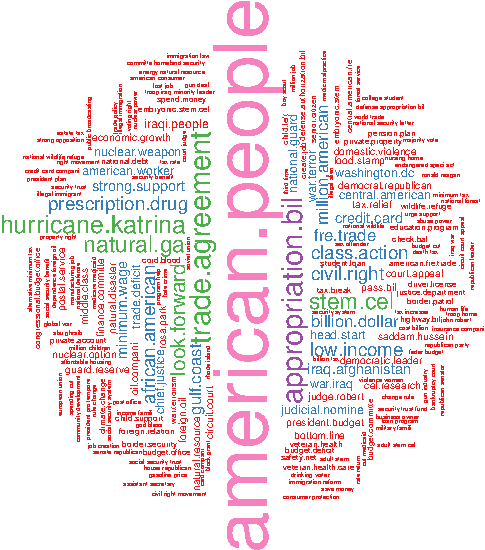
\includegraphics[scale=0.5]{figures/unnamed-chunk-3-1.pdf}
              
 \end{figure}


\end{frame}
%----------------------------------------------------------------------%
\begin{frame}[fragile]
\frametitle{Text Regression: Wordle (Wordclouds)}


\begin{scriptsize}


\begin{Shaded}
\begin{Highlighting}[]
\KeywordTok{tail}\NormalTok{(}\KeywordTok{colSums}\NormalTok{(congress109Counts))}
\end{Highlighting}
\end{Shaded}
\end{scriptsize}
\begin{tiny}



\begin{verbatim}
##          stem.cel        natural.ga hurricane.katrina   trade.agreement 
##              1699              1792              2020              2329 
## appropriation.bil   american.people 
##              2357              6256
\end{verbatim}
\end{tiny}

\begin{scriptsize}



\begin{Shaded}
\begin{Highlighting}[]
\KeywordTok{wordcloud}\NormalTok{(}\DataTypeTok{words =} \KeywordTok{colnames}\NormalTok{(congress109Counts), }
          \DataTypeTok{freq =} \KeywordTok{colSums}\NormalTok{(congress109Counts),}
          \DataTypeTok{min.freq =} \DecValTok{1000}\NormalTok{, }
          \DataTypeTok{scale =} \KeywordTok{c}\NormalTok{(}\DecValTok{3}\NormalTok{, }\FloatTok{0.1}\NormalTok{), }\DataTypeTok{max.words=}\DecValTok{30}\NormalTok{, }
          \DataTypeTok{random.order=}\OtherTok{FALSE}\NormalTok{, }\DataTypeTok{rot.per=}\FloatTok{0.35}\NormalTok{, }
          \DataTypeTok{colors=}\KeywordTok{brewer.pal}\NormalTok{(}\DecValTok{8}\NormalTok{, }\StringTok{"Set1"}\NormalTok{))}
\end{Highlighting}
\end{Shaded}

\end{scriptsize}


  \begin{figure}[H] \centering
            \captionsetup{justification=centering}
              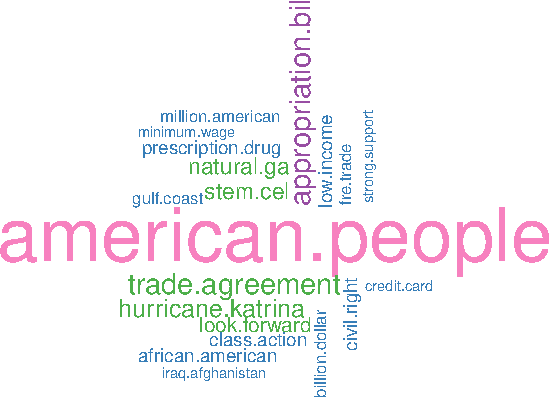
\includegraphics[scale=0.5]{figures/unnamed-chunk-5-1.pdf}
              
 \end{figure}



\end{frame}
%----------------------------------------------------------------------%
\begin{frame}[fragile]
\frametitle{Text Regression}

\begin{itemize}
  \item We can use {\tt LASSO}
\end{itemize}
\begin{scriptsize}

\begin{Shaded}
\begin{Highlighting}[]
\NormalTok{f \textless{}{-}}\StringTok{ }\NormalTok{congress109Counts}
\NormalTok{y \textless{}{-}}\StringTok{ }\NormalTok{congress109Ideology}\OperatorTok{$}\NormalTok{repshare}
\CommentTok{\# lasso }
\NormalTok{lassoslant \textless{}{-}}\StringTok{ }\KeywordTok{cv.gamlr}\NormalTok{(congress109Counts}\OperatorTok{\textgreater{}}\DecValTok{0}\NormalTok{, y)}
\NormalTok{B \textless{}{-}}\StringTok{ }\KeywordTok{coef}\NormalTok{(lassoslant}\OperatorTok{$}\NormalTok{gamlr)[}\OperatorTok{{-}}\DecValTok{1}\NormalTok{,]}
\KeywordTok{head}\NormalTok{(}\KeywordTok{sort}\NormalTok{(}\KeywordTok{round}\NormalTok{(B[B}\OperatorTok{!=}\DecValTok{0}\NormalTok{],}\DecValTok{4}\NormalTok{)),}\DecValTok{10}\NormalTok{)}
\end{Highlighting}
\end{Shaded}

\end{scriptsize}
\begin{tiny}


\begin{verbatim}
##    congressional.black.caucu                 family.value 
##                      -0.0839                      -0.0443 
##        issue.facing.american           voter.registration 
##                      -0.0324                      -0.0298 
##      minority.owned.business            strong.opposition 
##                      -0.0284                      -0.0264 
##                  civil.right        universal.health.care 
##                      -0.0259                      -0.0254 
## congressional.hispanic.caucu          ohio.electoral.vote 
##                      -0.0187                      -0.0183
\end{verbatim}
\end{tiny}

\end{frame}
%----------------------------------------------------------------------%
\begin{frame}[fragile]
\frametitle{Text Regression}

\begin{scriptsize}

\begin{Shaded}
\begin{Highlighting}[]
\KeywordTok{tail}\NormalTok{(}\KeywordTok{sort}\NormalTok{(}\KeywordTok{round}\NormalTok{(B[B}\OperatorTok{!=}\DecValTok{0}\NormalTok{],}\DecValTok{4}\NormalTok{)),}\DecValTok{10}\NormalTok{)}
\end{Highlighting}
\end{Shaded}

\end{scriptsize}
\begin{tiny}

\begin{verbatim}
##         illegal.alien        percent.growth   illegal.immigration 
##                0.0079                0.0083                0.0087 
##            global.war          look.forward            war.terror 
##                0.0098                0.0099                0.0114 
##      private.property        action.lawsuit          human.embryo 
##                0.0133                0.0142                0.0226 
## million.illegal.alien 
##                0.0328
\end{verbatim}


\end{tiny}

\end{frame}




%----------------------------------------------------------------------%
%----------------------------------------------------------------------%
\end{document}
%----------------------------------------------------------------------%
%----------------------------------------------------------------------%

